\documentclass[10pt,a4paper]{report}
\usepackage[utf8]{inputenc}
\usepackage{amsmath}
\usepackage{amsfonts}
\usepackage{amssymb}
\usepackage{ragged2e}
\usepackage{graphicx}
\usepackage{fixltx2e}
\usepackage{multicol}
\usepackage{tabularx}
\usepackage{tikz}
\usetikzlibrary{arrows,shapes,automata,petri,positioning,calc}
\usepackage{hyperref}
\hypersetup{
    colorlinks=true,
    linkcolor=blue,
    filecolor=magenta,      
    urlcolor=blue,
    }
\usepackage{tikz}
\usetikzlibrary{matrix,calc}
\usepackage[margin=0.5in]{geometry}
\providecommand{\norm}[1]{\left\lVert#1\right\rVert}
\newcommand{\myvec}[1]{\ensuremath{\begin{pmatrix}#1\end{pmatrix}}}
\let\vec\mathbf
\newcommand{\mydet}[1]{\ensuremath{\begin{vmatrix}#1\end{vmatrix}}}
\providecommand{\mtx}[1]{\mathbf{#1}}
\newenvironment{Figure}
  {\par\medskip\noindent\minipage{\linewidth}}
  {\endminipage\par\medskip}
\begin{document}
\begin{figure*}[!tbp]
  \centering
  \begin{minipage}[b]{0.4\textwidth}
   
\includegraphics[scale=0.05]{IITH-logo.jpg} 
  \end{minipage}
  \hfill
  \vspace{5mm}\begin{minipage}[b]{0.4\textwidth}
\raggedleft 
\includegraphics[scale=0.6]{nrc.jpeg} 
  \end{minipage}\vspace{0.2cm}
\end{figure*}
\raggedright \textbf{Name}:\hspace{1mm}Syed Tabasum nazeer\hspace{3cm} \Large \textbf{Line Assignment}\hspace{2.5cm} % 
\normalsize \textbf{Roll No.} :\hspace{1mm} FWC22093\vspace{1cm}
\begin{multicols}{2}
\raggedright \textbf{Problem Statement:}\vspace{2mm}
\raggedright \\The incentre of the triangle with vertices (1,$\sqrt{3}$), (0,0) and (2,0) is:

(a)(1,$\sqrt{3}$/2) \hspace{2cm} (b)(2/3,1/$\sqrt{3}$) 

(c)(2/3,$\sqrt{3}$/2) \hspace{2cm}  (d)(1,1/$\sqrt{3}$)\\
\vspace{5mm}
 \vspace{2mm} 
 \textbf{Construction:}
\begin{center}
\setlength{\arrayrulewidth}{0.5mm}
\setlength{\tabcolsep}{6pt}
\renewcommand{\arraystretch}{1.5}
    \begin{tabular}{|l|c|} \hline
    \textbf{vertex} & \textbf{coordinates} \\ \hline
   A & $ \begin{pmatrix} 
1 \\
\sqrt{3}
\end{pmatrix} $ \\ \hline
   B & $ \begin{pmatrix} 
0 \\
0
\end{pmatrix} $ \\ \hline  
   C & $ \begin{pmatrix} 
2 \\
0
\end{pmatrix} $ \\ \hline
      \end{tabular}
  \end{center}
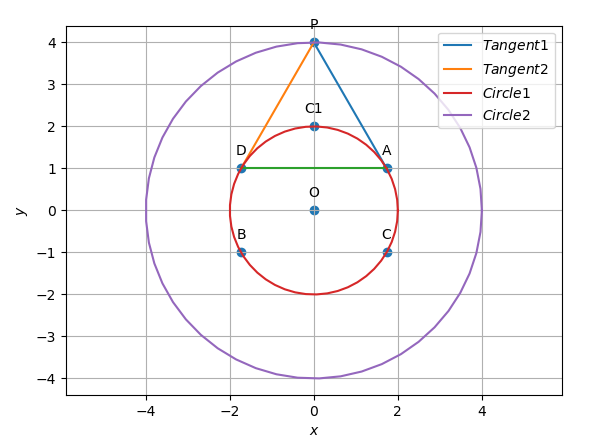
\includegraphics[scale=0.4]{Picture.png}
\\
\textbf{Step1:} With the given vertices form a triangle ABC
\newline
\\
\textbf{Step2:} Let AD is the angular bisector of angle A, then D divides BC in the ratio of AB:AC. Find point D and join AD.
\newline
\\
\textbf{Step3:} Let BE is the angular bisector of angle B, then E divides AC in the ratio of AB:BC. Find point E and join BE.
\newline
\\
\textbf{Step4:} Let CF is the angular bisector of angle C, then F divides AB in the ratio of AC:BC. Find point F and join CF.
\newline
\\
\textbf{Step5:} Finding out the point of intersection of any two angular bisectors gives the incentre of triangle ABC.
\newline
\\
Python code to find incenter of triangle can be downloaded from the following link.
\\
\vspace{2mm} 
\boxed{\href{https://github.com/SyedTabassumNazeer/FWC}{https://github.com/SyedTabassumNazeer/FWC}.}
\\
\vspace{2mm}
\textbf{Solution1:}
The vectors for the linesegments AB,BC and CA  are   \\
\begin{equation}
\vec{V_1} = \vec{A}-\vec{B}
\end{equation}\\
\begin{equation}
\vec{V_2} = \vec{B}-\vec{C}
\end{equation}\\
\begin{equation}
\vec{V_3} = \vec{A}-\vec{C}
\end{equation} \\
\vspace{2mm}
\hspace{1cm} Norms of the vectors V1, V2 and V3 are 
\begin{align}
\norm{\vec{V_1}}=2
\end{align}
\begin{align}
\norm{\vec{V_2}}=2
\end{align}
\begin{align}
\norm{\vec{V_3}}=2
\end{align}
\hspace{1.6cm} The incenter of a triangle is given by,
\begin{align}
\boxed{\vec{I}=\frac{\norm{\vec{V_1}}{\vec{C}}+\norm{\vec{V_2}}{\vec{A}}+\norm{\vec{V_3}}{\vec{B}}}{\norm{\vec{V_1}}+\norm{\vec{V_2}}+\norm{\vec{V_3}}}}
\end{align}
%\begin{align}
%\vec{I}=\frac{2({\vec{2i}})+2({\vec{i+\sqrt{3}j}})+2({\vec{0}})}{2+2+2}
%\end{align}
%\begin{align}
%\vec{I}=\frac{\vec{6i+2\sqrt{3}j}}{6}
%\end{align}	
%\begin{align}
%\vec{I}=\vec{i+j(\frac{1}{\sqrt{3}})}
%\end{align}
On substituting the values, we get incentre as
\newline	 
\begin{align}
\boxed{\vec{I=(1,\frac{1}{\sqrt{3}})}}
\end{align}
\textbf{Solution2:}
\justify{By the definition, incentre of a triangle is a point at which all the angular bisectors intersect.}
\newline
\textbf{Step1:} Let AD be the angular bisector of angle A. The point D divides BC in the ratio of $\frac{V_1}{V_3}$ (i;e $\frac{BD}{DC}$ = $\frac{V_1}{V_3}$). Then D is given by the equation
\begin{align}
 \vec{D = \frac{\norm{V_3}(B)+\norm{V_1}(C)}{\norm{V_1}+\norm{V_3}}}
\end{align}
%\begin{align}
% \vec{D} = \frac{2(0)+2(2\vec{i})}{2+2}
%\end{align}
%\begin{align}
%\vec{D = i}
%\end{align}\\
\textbf{Step2:} Let BE be the angular bisector of angle B. The point E divides AC in the ratio of $\frac{V_1}{V_2}$ (i;e $\frac{AE}{EC}$ = $\frac{V_1}{V_2}$). Then E is given by the equation
\begin{align}
 \vec{E = \frac{\norm{V_2}(A)+\norm{V_1}(C)}{\norm{V_1}+\norm{V_2}}}
\end{align}
%\begin{align}
%\vec{E} = \frac{2(\vec{i}+\sqrt{3}\vec{j})+2(2\vec{i})}{2+2}
%\end{align}
%\begin{align}
%\vec{E} = \frac{6\vec{i}+2\sqrt{3}\vec{j}}{4}
%\end{align}
%\textbf{Step3:} Let CF be the angular bisector of angle C. The point F divides AB in the ratio of $\frac{V3}{V2}$ (i;e $\frac{AF}{FB}$ = $\frac{V3}{V2}$). Then F is given by the equation
\begin{align}
 \vec{F = \frac{\norm{V_2}(A)+\norm{V_3}(B)}{\norm{V_2}+\norm{V_3}}}
\end{align}
%\begin{align}
 %\vec{F} = \frac{2(\vec{i}+\sqrt{3}\vec{j})+2(0)}{2+2}
%\end{align}
%\begin{align}
%\vec{F} = \frac{\vec{i}+\sqrt{3}\vec{j}}{2}
%\end{align}
\textbf{Step4:} The line equation of the angular bisector AD is given by
\begin{align}
\vec{G} = \vec{A} + \lambda1\vec{(D-A)}
\end{align}
%\begin{align}
%\vec{G} =  \vec{i}+\sqrt{3}\vec{j}+ \lambda1(\vec{i}-(\vec{i}+\sqrt{3}\vec{j}))
%\end{align}
%\begin{align}
%\vec{G} = \vec{i} + (1-\lambda1)\sqrt{3}\vec{j}
%\end{align}
\textbf{Step5:} The line equation of the angular bisector BE is given by
\begin{align}
\vec{H} = \vec{B} + \lambda2(\vec{E-B})
\end{align}
%\begin{align}
%\vec{H} =  0 + \lambda2((\frac{6\vec{i}+2\sqrt{3}\vec{j}}{4})-0)
%\end{align}
%\begin{align}
%\vec{H} = \vec{i}(\frac{3}{2}\lambda2) + \vec{j}(\frac{\sqrt{3}}{2}\lambda2)
%\end{align}
%\textbf{Step6:} The point of intersection of the angular bisector G and H gives the %incentre of the triangle. At the point of intersection of two vectors, the coefficients of components $\vec{i}$, $\vec{j}$, $\vec{k}$ becomes equal. 
%\begin{align}
%\vec{G} = \vec{i} + (1-\lambda1)\sqrt{3}\vec{j}
%\end{align}
%\begin{align}
%\vec{H} = \vec{i}(\frac{3}{2}\lambda2) + \vec{j}(\frac{\sqrt{3}}{2}\lambda2)
%\end{align}
%On equating coefficients of $\vec{i}$ component of G and H we get
%\begin{align}
%\frac{3}{2}\lambda2 = 1
%\end{align}
%\begin{align}
%\boxed{\lambda2 = \frac{2}{3}}
%\end{align}
%On equating coefficients of $\vec{j}$ component of G and H we get
%\begin{align}
%\sqrt{3}(1-\lambda1) = \frac{\sqrt{3}}{2}\lambda2
%\end{align}
%\begin{align}
%1-\lambda1 = \frac{1}{2}\lambda2
%\end{align}
%\begin{align}
%1-\lambda1 = \frac{1}{2}(\frac{2}{3})
%\end{align}
%\begin{align}
%1-\lambda1 = \frac{1}{3}
%\end{align}
%\begin{align}
%\boxed{\lambda1 = \frac{2}{3}}
%\end{align}
\textbf{Step6:} On solving G and H we get the values of $\lambda1$ and $\lambda2$. On sustituting $\lambda1$ in G we get the point of intersection of angular bisectors,i;e Incentre
%\begin{align}
%\vec{G} = \vec{i} + (1-\frac{2}{3})\sqrt{3}\vec{j}
%\%end{align}
%\begin{align}
%= \vec{i} + (\frac{1}{\sqrt{3}})\vec{j}
%\end{align}
\begin{align}
\boxed{Incentre = (1,\frac{1}{\sqrt{3}})}
\end{align}
\newline
\textbf{Solution3:}
\justify{From the solution1, it is clear that the given triangle is a equilateral triangle (i;e V1 = V2 = V3). One of the property of the eqilateral triangle is that the incentre of the triangle is same as the centroid.  The centroid of the triangle is given by,}
\begin{equation}
Centroid = \frac{\vec{A+B+C}}{3}
\end{equation}
%\begin{equation}
%= \frac{\vec{i}+\sqrt{3}\vec{j}+2\vec{i}}{3}
%\end{equation}
%\begin{equation}
%= \frac{3\vec{i}+\sqrt{3}\vec{j}}{3}
%\end{equation} \
\begin{align}
Centroid=\vec{(1,\frac{1}{\sqrt{3}})}
\end{align}
\begin{align} 
\boxed{Centroid={Incenter}}
\end{align}
Hence, centroid of an equilateral triangle is equal to the Incentre of the triangle
\end{multicols}
\end{document}